\DiaryEntry{Scalar Quantization, 1}{2021-06-15}{Coding}

Quantization can be seen as lossy compression method as a large (potentially infinite) number of values is represented by (much) fewer values. If the values we are looking at are scalars, the process is called scalar quantization and that's what we are looking at here.

The quantizer design process can be conceptualized (and is often implemented) as consisting of two steps: In the first step, the set of all values taken on by the source is partitioned. In the second step all the values in a partition are represented by a single value. Because we will represent a set of values by a single value, this process necessarily results in the loss of information. How we measure this loss is an important factor in the design of the quantizer and affects the shape of the partitions. How many bits we will use to represent the output of the quantizer, in most cases, determines the number of partitions.

\subsection{Introduction}

\paragraph{Definitions.} A quantizer $Q$ takes a real-valued input $x$, checks into which of the $M$ partitions it falls into and assigns it to one of $M$ representative output values called \emph{reconstruction levels}. The partitions are separated by $M-1$ \emph{decision boundaries}.

If we denote the decision boundaries with $b_i, i=0, \ldots M$ and the reconstruction levels with $y_i, i=1, \ldots, M$, then

\bee
y_i = Q(x) \quad \text{if} \,\, b_{i-1} < x \leq b_i
\eee

The following Figure shows an example of a quantizer. Decision boundaries are $-3, -2, \\ -1, 0, 1, 2, 3$ and reconstruction levels are $-3.5, -2.5, -1.5, -0.5, 0.5, 1.5, 2.5, 3.5$. An input value of $x = 1.4$ would yield a reconstruction value of $y = 1.5$.

\begin{figure}[H]
    \centering
    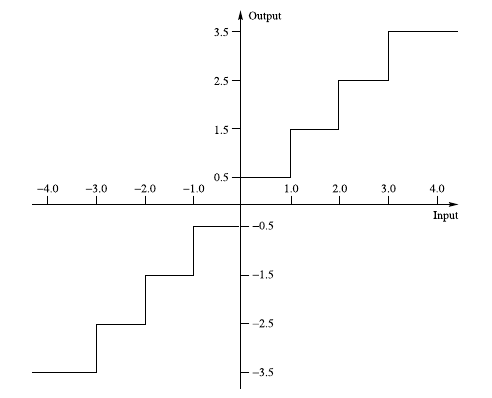
\includegraphics[scale=0.7]{images/2021-06-15-scalar_quant_01.png}
\end{figure}

Note that there is no representation for the input value zero; the quantizer is also called a \emph{midrise quantizer}. If there were a representation for zero, it would be a \emph{midtread quantizer}.

As the midtread quantizer has zero as one of its output levels, it is especially useful in situations where it is important that the zero value be represented; for example, control systems in which it is important to represent a zero value accurately, and audio coding schemes in which we need to represent silence periods.

We assess the quantization error $\sigma_q^2$ in terms of mean squared error; if we denote the pdf of $x$ with $f_X(x)$, we have

\bee
\sigma_q^2 = \int_{- \infty}^\infty (x - Q(x))^2 f_X(x) dx = \sum_i \int_{b_{i-1}}^{b_i} (x - y_i)^2 f_X(x) dx
\eee

The difference between the quantizer input $x$ and output $y = Q(x)$, besides being referred to as the quantization error, is also called the quantizer distortion or quantization noise. But the word “noise” is somewhat of a misnomer. Generally, when we talk about noise we mean a process external to the source process. Because of the manner in which the quantization error is generated, it is dependent on the source process and, therefore, cannot be regarded as external to the source process.

If we use fixed-length codewords to represent the quantizer output, then the size of the output alphabet immediately specifies the rate. If the number of quantizer outputs is $M$, then the rate is given by

\bee
R = \lceil \log_2 M \rceil
\eee

However, if we are allowed to use variable-length codes, such as Huffman codes or arithmetic codes, along with the size of the alphabet, the selection of the decision boundaries will also affect the rate of the quantizer. If $l_i$ is the codeword length of output $y_i$ and $P(y_i)$ is the corresponding probability of $y_i$, then the rate becomes

\bee
R = \sum_i l_i P(y_i) = \sum_i l_i \int_{b_{i-1}}^{b_i} f_X(x) dx
\eee

From this we see that for a given source input, the partitions we select and the representation for those partitions will determine the distortion incurred during the quantization process. The partitions we select and the binary codes for the partitions will determine the rate for the quantizer. Thus, the problem of finding the optimum partitions, codes, and representation levels are all linked.

\paragraph{Quantizer Design Problem.} There are two ways we can design the quantizer: First one is to define a distortion constraint $D^\star$ and seek a quantizer scheme (decision boundaries, representation levels, and binary codes) that minimize the rate $R$ while having $\sigma_q^2 \leq D^\star$. The other one is to define a rate constraint $R^\star$ and seek a quantizer scheme which minimizes the distortion $\sigma_q^2$.

\subsection{Uniform Quantizer}

The simplest type of quantizer is the uniform quantizer. All intervals are the same size in the uniform quantizer, except possibly for the two outer intervals. In other words, the decision boundaries are spaced evenly. The reconstruction values are also spaced evenly, with the same spacing as the decision boundaries; in the inner intervals, they are the midpoints of the intervals. This constant spacing is usually referred to as the step size $\Delta$. The quantizer shown in the Figure above is such a uniform quantizer.

\paragraph{Uniformly distributed Source.} This is the simplest case; Suppose we want to design an $M$-level uniform quantizer for an input signal which is uniformly distributed between $[-X_{max}, X_{max}]$. The stepsize therefore becomes

\bee
\Delta = \frac{2 X_{max}}{M}
\eee

and the distortion becomes

\bee
\sigma_q^2 = 2 \sum_{i=1}^{M/2} \int_{(i-1) \Delta}^{i \Delta} \left(x - \frac{2i-1}{2} \Delta \right)^2 \frac{1}{2 X_{max}} dx
\eee

This is not complicated but cumbersome. Instead we take a look at the quantization error $q$,

\bee
q = Q(x) - x
\eee

This is plotted below and looks much easier.

\begin{figure}[H]
    \centering
    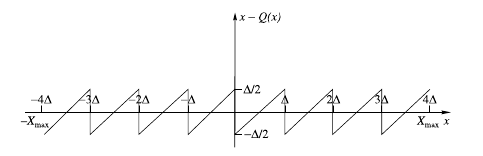
\includegraphics[scale=0.7]{images/2021-06-15-scalar_quant_02.png}
\end{figure}

As the input is uniform, the quantization error $q$ is also uniform in $[-\Delta/2, \Delta/2]$ and the calculation of the mean squared error simplifies todonotes

\bee
\sigma_q^2 = \frac{1}{\Delta } \int_{- \Delta/2}^{\Delta / 2} q^2 dq = \frac{\Delta^2}{12}
\eee

With this we can calculate the SNR. The "noise" power is $\sigma_q^2$. The signal power $\sigma_s^2$ of a uniformly distributed signal in $[-X_{max}, X_{max}]$ is given by

\bee
\sigma_s^2 = \frac{1}{2 X_{max}} \int_{-X_{max}}^{X_{max}} x^2 dx = \frac{1}{2 X_{max}} \left( \frac{X_{max}}{3} - - \frac{X_{max}}{3} \right) = \frac{X^2_{max}}{3}
\eee

In order to relate this to $\sigma_q^2$, we need a connection between $\Delta$ and $X_{max}$. If our quantizer has $M$ levels, we have

\bee
\Delta = \frac{2 X_{max}}{M}
\eee

and our "noise power becomes $\sigma_q^2 = \frac{4 X^2_{max}}{12 M^2}$. The SNR then becomes

\begin{align*}
    SNR(dB) &= 10 \log \frac{\sigma_s^2}{\sigma_q^2} \\
&= 10 \log \frac{ \frac{X^2_{max}}{3} }{ \frac{4 X^2_{max}}{12 M^2} } \\
&= 10 \log \frac{X^2_{max}}{3} \frac{12 M^2}{4 X^2_{max}} \\
&= 10 \log M^2 \\
&= 20 \log M \\
&= 20 \log 2^n \\
&= 20 n \log 2 \approx 6.02 n dB
\end{align*}

We have made use of the fact that the number of levels $M$ equals $2^n$ where $n$ is the number of bits $n$ the quantizer uses. The good thing is that the SNR does not depend on $X_{max}$ and it is a rather simple formula. Note that it depends on the assumption of the uniform quantizer and the uniformly distributed input signal.

\paragraph{Other Source Distributions.} We can write down the quantization noise (for a midrise quantizer) for arbitrary signal distributions as

\begin{align*}
    \sigma_q^2 = &2 \sum_{i=1}^{M/2-1} \int_{(i-1) \Delta}^{i \Delta} \left(x - \frac{2i-1}{2} \Delta \right)^2 \frac{1}{2 X_{max}} dx \\
    &+ 2 \int_{(M/2-1)\Delta}^{\infty} \left(x - \frac{M-1}{2} \Delta \right)^2 \frac{1}{2 X_{max}} dx
\end{align*}

To find the optimal value of $\Delta$, this expression can be differentiated wrt to $\Delta$, set to zero, and solved for $\Delta$ (at least numerically).

\paragraph{Mismatch.} There are two types of mismatch: The distribution parameters could be wrong (e.g. the uniform distribution has a different $X_{max}$ than the quantizer was designed for) or the distribution is actually a different one (e.g. using a quantizer designed for uniform input distribution with an input being distributed normally). Both cases lead to an increase in the MSE $\sigma_q^2$.

For example, we designed a quantizer for a uniform source with $X_{max} = 1$. If this source is used and the quantizer has $M = 8$ levels ($n = 3$ bits), then we observe an SNR of $6.02 \times 3 dB \approx 18dB$ as calculated above.

If $X_{max} = 0.8$, then the observed SNR becomes $15$dB, in case of $X_{max} = 0.5$, the observed SNR drops to  $12$dB.

We next used an input signal with normal distribution $(\Nc(0, \sigma_s^2)$ and designed the quantizer with $X_{max} = 1$. The following Figure shows the achieved SNR for over $\sigma_s^2$. The maximum SNR of about $19$dB is reached for $\sigma_s^2 \approx 0.5$ for lower and higher signal energies it falls off (rather rapidly). In case of low $\sigma_s^2$, the outer quantizer intervals are not used often enough and thereby leading a low SNR, in case of high $\sigma_s^2$, the innter quantizer intervals ar enot used often enough and the signal experiences clipping (also leading to a low SNR).

\begin{figure}[H]
    \centering
    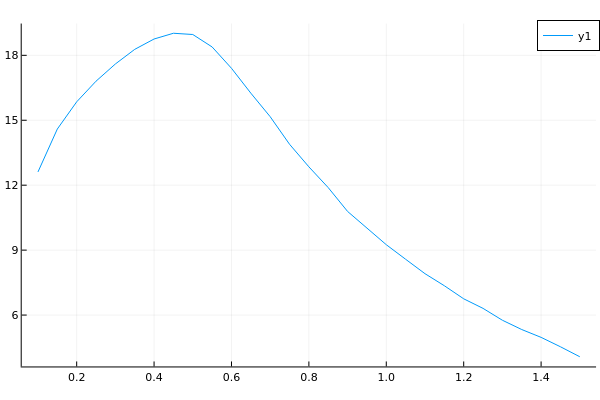
\includegraphics[scale=0.5]{images/2021-06-15-scalar_quant_03.png}
\end{figure}



If the input signal has a normal distribution $\Nc(0,1)$ instead of the $[-1, 1]$ uniform one the quantizer was designed for, then the SNR drops to $4.5$dB! The tails of the normal distribution cause a lot of clipping, leading to this bad result. Only if we decrease the variance and work with a $\Nc(0, 0.1)$ distrubtion, we get an SNR of about $17.9$dB again.

\subsection{Adaptive Quantization}

One way to deal with the mismatch problem is to adapt the quantizer to the statistics of the input.

There are two main approaches to adapting the quantizer parameters: an off-line or forward adaptive approach, and an on-line or backward adaptive approach. 

\paragraph{Forward Adaptive Quantization.} In forward adaptive quantization, the source output is divided into blocks of data. Each block is analyzed before quantization, and the quantizer parameters are set accordingly. The settings of the quantizer are then transmitted to the receiver as side information. In backward adaptive quantization, the adaptation is performed based on the quantizer output. As this is available to both transmitter and receiver, there is no need for side information.

This approach causes a delay of at least the amount of time required to process a block of data. The insertion of side information in the transmitted data stream may also require the resolution of some synchronization problems. The size of the block of data processed also affects a number of other things. If the size of the block is too large, then the adaptation process may not capture the changes taking place in the input statistics. Furthermore, large block sizes mean more delay, which may not be tolerable in certain applications. On the other hand, small block sizes mean that the side information has to be transmitted more often, which in turn means the amount of overhead per sample increases. The selection of the block size is a trade-off between the increase in side information necessitated by small block sizes and the loss of fidelity due to large block sizes . The variance estimation procedure is rather simple. At time $n$ we use a block of $N$ future samples to compute an estimate of the variance

\bee
\sigma_s^2 = \frac{1}{N} \sum_{i=0}^{N-1} x_{n+1}^2
\eee

Using this estimate, the quantizer is designed. The quatizer design parameters need also to be transmitted to the receiver.

\paragraph{Backward Adaptive Quantization.} In backward adaptive quantization, only the past quantized samples are available for use in adapting the quantizer. The values of the input are only known to the encoder; therefore, this information cannot be used to adapt the quantizer. How can we get information about mismatch simply by examining the output of the quantizer without knowing what the input was? If we studied the output of the quantizer for a long period of time, we could get some idea about mismatch from the distribution of output
values. If the quantizer step size $\Delta$ is well matched to the input, the probability that an input to the quantizer would land in a particular interval would be consistent with the pdf assumed for the input. However, if the actual pdf differs from the assumed pdf, the number of times the input falls in the different quantization intervals will be inconsistent with the assumed pdf. If $\Delta$ is smaller than what it should be, the input will fall in the outer levels of the quantizer an excessive number of times. On the other hand, if $\Delta$ is larger than it should be for a particular source, the input will fall in the inner levels an excessive number of times. 

This approach is used in \emph{Jayant quantizer}: If the input falls in the outer levels, the step size needs to be expanded; and if the input falls in the inner quantizer levels, the step size needs to be reduced. The expansions and contractions should be done in such a way that once the quantizer is matched to the input, the product of the expansions and contractions is unity. The 

The expansion and contraction of the step size is accomplished in the Jayant quantizer by assigning a multiplier $M_k$ to each interval. If the $n-1$th input falls in the $k$th interval, the step size to be used for the $n$th input is obtained by multiplying the step size used for the $n-1$th input with $M_k$. The multiplier values for the inner levels in the quantizer are less than one, and the multiplier values for the outer levels of the quantizer are greater than one. Therefore, if an input falls into the inner levels, the quantizer used to quantize the next input will have a smaller step size. Similarly, if an input falls into the outer levels, the step size will be multiplied with a value greater than one, and the next input will be quantized using a larger step size. Notice that the step size for the current input is modified based on the previous quantizer output. The previous quantizer output is available to both the transmitter and receiver, so there is no need to send any additional information to inform the receiver about the adaptation. 

Critical to the good performance of the Jayant quantizer is the choice of the multipliers (not covered here).


%%% Local Variables:
%%% mode: latex
%%% TeX-master: "journal"
%%% End:
